\chapter{実装}
\label{chap:jissou}

本章では第\ref{chap:sekkei}章で述べたシステムの設計を受け、DrawWikiの実装について述べる。

\newpage

\section{アプリケーション構成}
DrawWikiはWebアプリケーションとして実装されており、
HTML5とSVG1.1に準拠したブラウザがインストールされていれば、OSやデバイスに依存せず利用することができる。
本アプリケーションの構成は以下の図の通りである。

\begin{figure}[htbp]
    \begin{center}
        \fbox {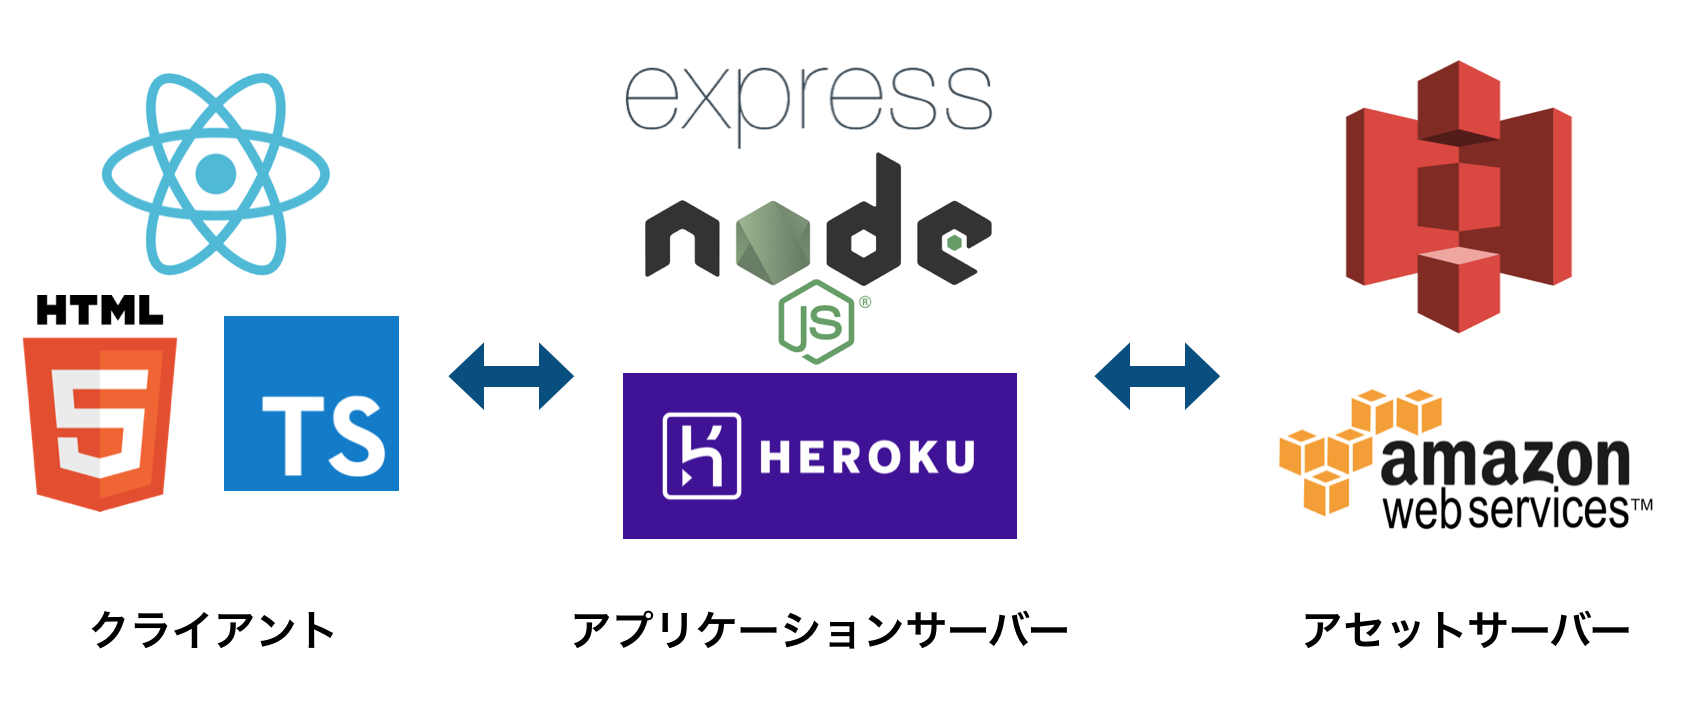
\includegraphics[width=110mm]{images/application.png}} \end{center}
    \caption{アプリケーションの構成}
\end{figure}

\section{クライアントサイド}
実際にハイパーイラストを作成したり関連イラストを閲覧したりするクライアントサイドのプログラムはHTML\footnote{https://developer.mozilla.org/ja/docs/Web/HTML}と
javascript\footnote{https://developer.mozilla.org/ja/docs/Glossary/JavaScript}によって実装される。
開発にはJavascriptにコンパイル可能な漸進的型付け言語TypeScript\footnote{https://www.typescriptlang.org/}を用いている。

\subsection{手書きデータの取得}
DrawWikiにおいて指やスタイラスの操作から生じる座標等の手書きデータをPointerEvent API\footnote{https://developer.mozilla.org/ja/docs/Web/API/PointerEvent}によって取得している。
このAPIはTouchEventやMouseEventと異なりタッチやマウスだけでなくスタイラスを含めたあらゆるユーザー入力を透過的に扱うことが可能で(図\ref{pevent})、
また主要なブラウザに全て実装されているためあらゆるプラットフォーム・デバイスから利用できる。

\begin{figure}[htbp] \begin{minipage}{0.5\hsize}
                         \begin{center}
                             \fbox {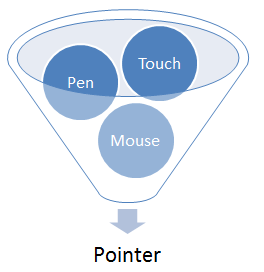
\includegraphics[width=50mm]{images/pevents.png}} \end{center}
                         \caption{PointerEvent APIの概要} \label{pevent}
\end{minipage} \begin{minipage}{0.5\hsize}
                            \begin{center}
                                \fbox {
\includegraphics[width=60mm]{images/testimage.png}} \end{center}
                            \caption{仮想DOMのモデル} \label{vdom}
\end{minipage}
\end{figure}

\subsection{仮想DOMの利用}
DrawWikiは大量に発生するPointerEventから動的に手書きストロークを生成し、ハイパーイラストを作成・描画するが、
単に描画するだけでなく内部の任意の要素にハイパーリンクを埋め込んだり、別のハイパーイラストをインポートしたり等の複雑な操作を行うことがある。
例えばハイパーリンクを追加する際は以下のような処理を実行している。
\begin{enumerate}
    \item 範囲選択された座標内にあるストロークをSVGGroup要素で囲う
    \item グループ化したストローク群をさらにSVGAnker要素で囲う
    \item SVGAnker要素のhref属性にリンクさせるハイパーイラストのURLを代入する
\end{enumerate}
ハイパーイラストはベースとなるSVGと同様にあらゆる要素が階層構造的に記述されており、そのようなツリーの操作はDOMインターフェース
%URLにunderScoreが含まれているとビルドが通らない?
%\footnote{ \textsf{https://developer.mozilla.org/ja/docs/Web/API/Document_Object_Model/Introduction} }
(appendChildやremoveChild、insertBefore等)を通じて行うことが一般的である。

しかし例のような要素が階層構造内を横断するような複雑な処理をDOMインターフェースのみで行うことはコードの複雑化と描画パフォーマンスの低下を招く。
そこでDrawWikiでは実際のDOMを操作するのではなく、仮想DOMに対してのみ操作を行い、その差分を実際のDOMにDispatchする手法を用いている。
仮想DOMを実際のハイパーイラストに反映する処理はViewライブラリのReact\footnote{https://ja.reactjs.org/}を利用している。

\subsection{debounceされた更新処理}
DrawWikiではハイパーイラストが編集され変更が生じる度に自動でデータを上書き保存する仕様だが、画面上で指やスタイラスペンを動かしている間は
常にPointerEventが発生し続けているため、このまま変更をアップロードするとサーバー側の処理能力を超える頻度でリクエストを送信してしまう。
そこでEvent発生後にタイマーをセットし、2秒経過した段階でアップロード処理を行うdebounce機能を実装した。このタイマーは新しいEventが
発生する度にリセットされるため、ペンを置いてしばらく、つまり最後のEventから2秒間新たなEventが発生しないことが確定してからアップロード処理が行われる。
これによりアプリケーションサーバーやアセットサーバーに過大な負荷を与えることなく更新処理を行うことができる。


\subsection{リンク付要素の視覚的表現}
関連イラスト表示にはリンクしているハイパーイラストのサムネイルが表示されるが、
そのサムネイルを選択すると、そのハイパーイラストをリンクされている要素が変化し、対応関係が視覚的に表示される。
ハイパーイラストのベースとなるSVGはCSS\footnote{https://developer.mozilla.org/ja/docs/Web/CSS}を適用可能であり、
この視覚効果もCSSとCSS @keyframes\footnote{https://developer.mozilla.org/ja/docs/Web/CSS/@keyframes}を組み合わせることで実現している。

\section{サーバーサイド}
サーバーサイドはアプリケーションサーバーとアセットサーバーとで構成されている。

\subsection{アプリケーションサーバー}
DrawWikiはNode.js\footnote{https://nodejs.org/}上で動作するWebアプリケーションとして実装されている。
HTTPリクエストを処理するWebアプリケーションフレームワークとしてExpress\footnote{https://expressjs.com/}を用い、
そのホスティング環境としてBaaS(Backend-as-a-Service)の一つであるHeroku\footnote{https://www.heroku.com/}を利用している。

\subsubsection{ハイパーイラストのアップロード処理}
クライアントは作成したハイパーイラストを"multipart/form-data"形式でエンコーディングし、アプリケーションサーバーは
そのデータをPOST通信で受け取る。受け取ったハイパーイラストをもとにメタデータを生成し、双方をアセットサーバーに送信する
ことでアップロード処理を行う。

また既存のハイパーイラストや付随するメタデータの読み取り、更新、削除についてはREST原則\cite{Fielding2000ArchitecturalSA}
に基づいたルーティングによって処理する構成となっている。

\subsubsection{メタデータの構成}
ハイパーイラストの本体とは別に、以下のようなメタ情報を管理するためにDrawWikiではメタデータファイルも扱う。
\begin{itemize}
    \item ハイパーイラストの作成者
    \item 最終更新日時
    \item 引用している、またはインポートしているハイパーイラストのリスト
\end{itemize}

\begin{lstlisting}[caption=メタデータの概要, label=metadatajson]
    export type HyperIllust = {
    id: string; //ハイパーイラストのID
    sourceKey: string; //ハイパーイラストの本体ファイルのKey
    sourceURL: string;  //ハイパーイラストの本体ファイルのURL
    size?: number;  //ファイルサイズ
    linkedList?: string[];  //リンクされているハイパーイラストのリスト
    linkedByList?: string[];    //このイラストをリンクしているハイパーイラストのリスト
    importedList?: string[];    //インポートしたハイパーイラストのリスト
    importedByList?: string[];  //このイラストをインポートするハイパーイラストのリスト
    createdAt: DateLike;    //作成日時
    updatedAt: DateLike;    //更新日時
    owner: string;  //作成者の名前
    };
\end{lstlisting}

\subsection{アセットサーバー}
アプリケーションサーバーはステートレスなプロセスとして実行されるため、変数やファイル等を保存し永続化する仕組みをもたない。
ファイルとしてのハイパーイラストやメタデータを保存するためにDraWikiはアセットサーバーとして
クラウドストレージであるAWS S3\footnote{https://aws.amazon.com/jp/s3/}を利用している。
アップロードされたハイパーイラストはDrawWiki以外のWebサイトからも閲覧・再利用できるように、ACL(Access-Control-List)を
公開読み取り("public-read")に設定している。またアセットサーバー自体もオリジン間リソース共有\footnote{https://developer.mozilla.org/ja/docs/Web/HTTP/CORS}
を有効化している。
